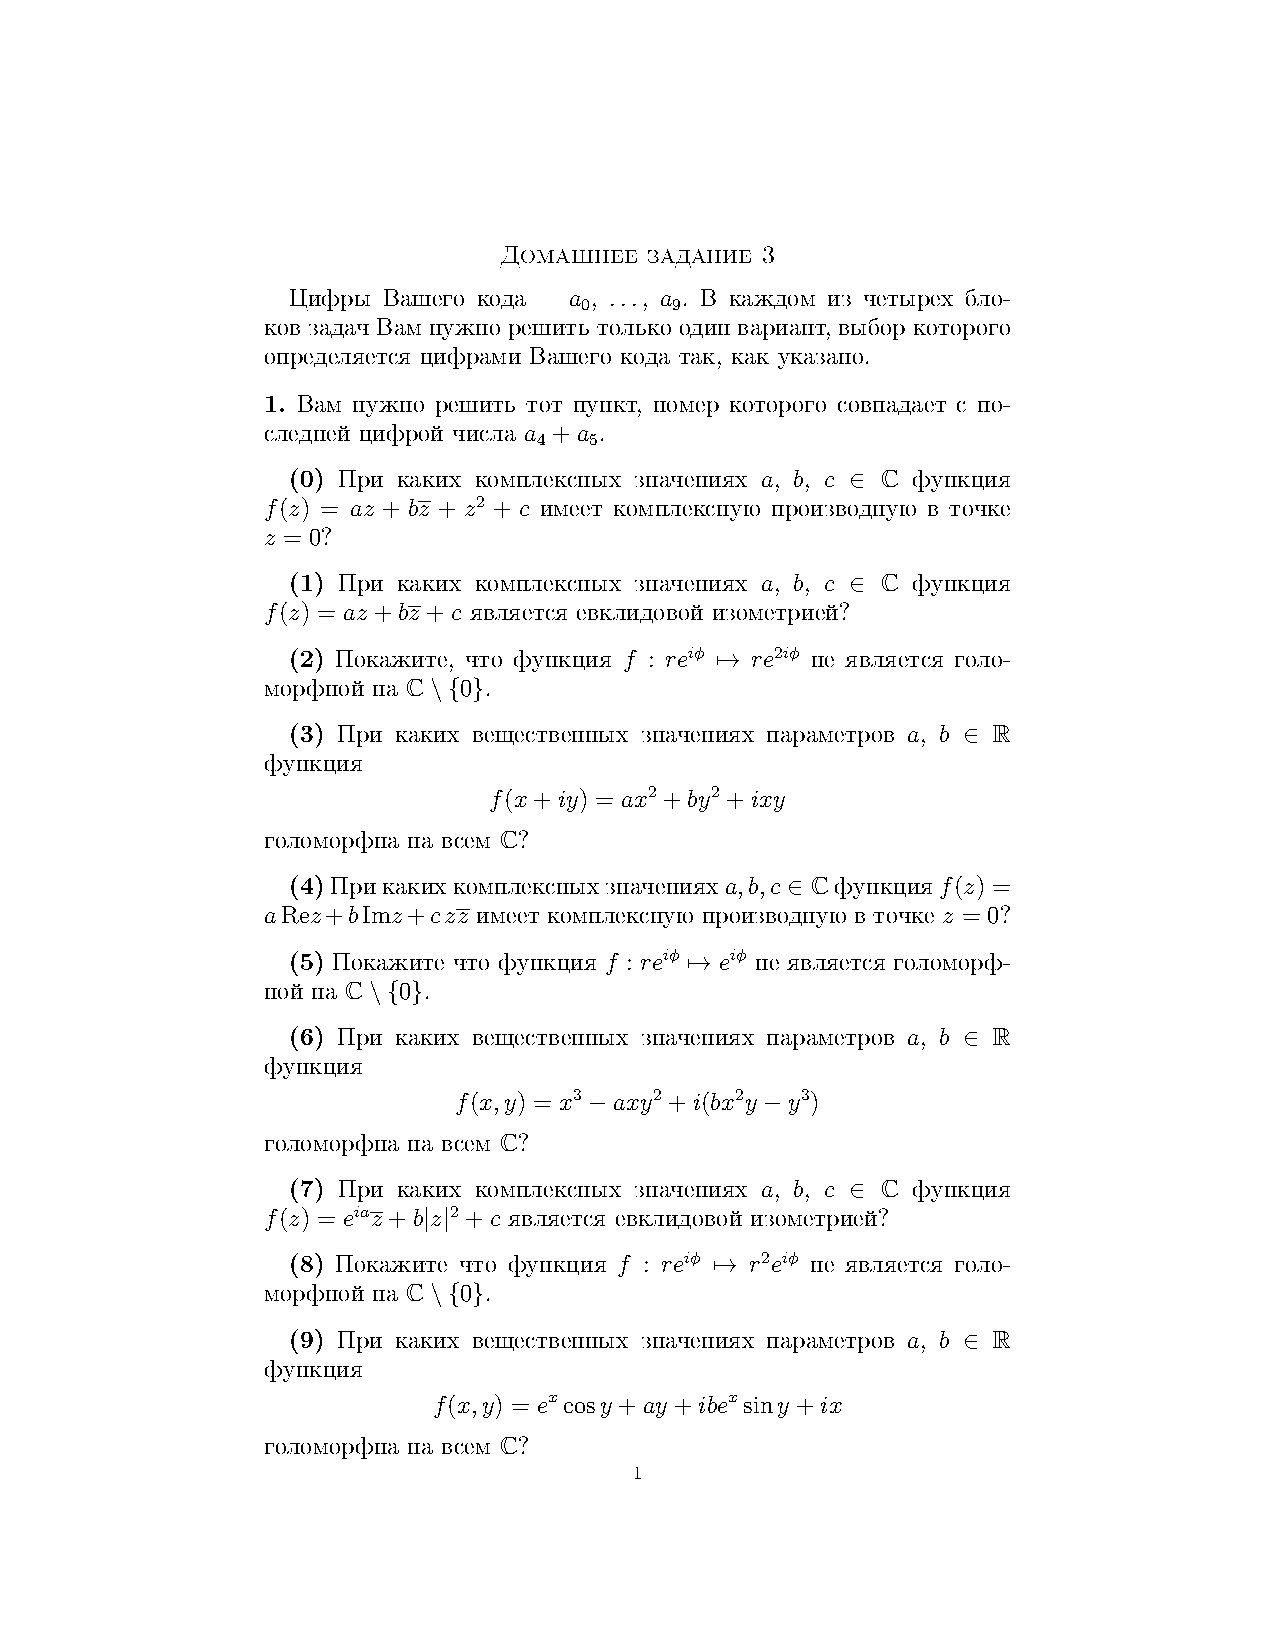
\includepdf[scale=1,pages=1-4]{Tasks/hw3}
\newpage
\section*{Решения}
\subsection*{Задача 1}
	Необходимо решить задачу $a_4 + a_5 = 7 + 6 = 3 \mod 10$
	\begin{gather*}
		f(x + iy) = u(x,y) + iv(x,y) = ax^2 + by^2 + ixy\\
		u(x,y) = ax^2 + b^2y\qquad v(x,y) = xy\\
		\frac{\partial u}{\partial x} = 2ax\qquad \frac{\partial u}{\partial y} = 2by\\
		\frac{\partial v}{\partial x} = y\qquad \frac{\partial v}{\partial y} = x
	\end{gather*}
	Каждая голоморфная функция удовлетворяет условиям Коши-Римана
	\begin{gather*}
		\frac{\partial u}{\partial x} = \frac{\partial v}{\partial y}\qquad \frac{\partial u}{\partial y} = -\frac{\partial v}{\partial x}
	\end{gather*}
	Откуда
	\begin{gather*}
		2ax = x\qquad 2by = -y\\
		a = \frac{1}{2}\qquad b = -\frac{1}{2}
	\end{gather*}
\vskip 0.4in

\subsection*{Задача 2}
	Необходимо решить задачу $a_3 + a_6 = 9 + 9 = 8 \mod 10$
	\begin{gather*}
		f:\ \mathbb{C} \backslash [-1,1] \to \mathbb{C}\\
		f:\ x + iy \to u(x,y) + i v(x,y)\\
		f(z^2) = z^2 - 1\qquad f(x^2 + 2ixy - y^2) = (x^2 - y^2 - 1) + i(2xy)\\
		f((x^2 - y^2) + i(2xy)) = (\Re(z^2) - 1) + i(\Im(z^2))
	\end{gather*}
	Утверждение: $\forall\ z = a + bi\ \exists !$ пара $x,y: \begin{cases} a = x^2 - y^2\\ b = 2xy \end{cases}$ и $\Im(f(i)) > 0\ b > 0$
	\vskip 0.1in
	Решим систему
	\begin{gather*}
	a = \frac{b^2}{4y^2} - y^2\\
	4y^4 + 4ay^2 - b^2 = 0\\
	D = 16a^2 + 16b^2 = 16|z|^2\\
	y^2 = \frac{-4a \pm 4|z|}{8} = \frac{-a \pm |z|}{2}\\
	b > 0 \Rightarrow |z| > a\\
	y = \sqrt{\frac{-a+|z|}{2}}\qquad
	x = \frac{b}{\sqrt{2(|z| - a)}}
	\end{gather*}
	Однозначно восстановили отображение
	$f:\ a+bi \mapsto a-1 + ib$
	оно единственно
\vskip 0.4in

\subsection*{Задача 3}
	Необходимо решить задачу $a_2 + a_7 = 8 + 3 = 1 \mod 10$
	\begin{gather*}
		\frac{\partial u}{\partial x} = e^x \cos(y)\qquad
		\frac{\partial^2 u}{\partial x^2} = e^x \cos(y)\\
		\frac{\partial u}{\partial y} = -e^x \sin(y)\qquad
		\frac{\partial^2 u}{\partial y^2} = -e^x \cos(y)\\
		\frac{\partial^2 u}{\partial x^2} + \frac{\partial^2 u}{\partial y^2} = e^x \cos(y) - e^x \cos(y) = 0
	\end{gather*}
	Следовательно $e^x \cos(y)$ -- гармоническая
	\begin{gather*}
		\frac{\partial u}{\partial x} = e^x \sin(y) = \frac{\partial v}{\partial y}\\
		\frac{\partial u}{\partial y} = e^x \cos(y) = -\frac{\partial v}{\partial x}\\
		v(x,y) = -e^x \cos(y) + \phi(x)\\
		e^x \cos(y) = e^x \cos(y) - \phi'(x)\\
		v(x,y) = -e^x \cos(y) + c
	\end{gather*}
\vskip 0.4in

\subsection*{Задача 4}
	Необходимо решить задачу $a_1 + a_8 = 7 + 8 = 5 \mod 10$\\
	Докажем более общий факт, что если $a \Re(f(z)) + b \Im(f(z)) = c$ при $a^2 + b^2 \ne 0$, то $f$ -- константа
	\begin{gather*}
		\Re(f) = u(x,y)\qquad \Im(f) = v(x,y)\\
		au(x,y) + bv(x,y) = c\\
		au_x + bv_x = 0\quad au_y + bv_y = 0\quad \text{диффиринцирование с обеих сторон}\\
		au_x - bu_y = 0\quad au_y + bu_x = 0\quad \text{условия Коши-Римана}\\
		\begin{pmatrix}
			a & -b \\ b & a
		\end{pmatrix}
		\begin{pmatrix}
			u_x \\ u_y
		\end{pmatrix}
		=
		\begin{pmatrix}
			0 \\ 0
		\end{pmatrix}\\
		\begin{vmatrix}
			a & -b \\ b & a
		\end{vmatrix}
		= a^2 + b^2 \ne 0\\
		\begin{pmatrix}
			u_x \\ u_y
		\end{pmatrix}
		=
		\begin{pmatrix}
			0 \\ 0
		\end{pmatrix}\\
		v_x = v_y = 0\quad \text{то есть фугкция константа}
	\end{gather*}
\vskip 0.4in

\subsection*{Задача 5}
	Необходимо решить задачу $a_0 + a_9 = 1 + 6 = 7 \mod 10$\\
	Рассмотрим $f(z) = \sqrt{|xy|}$
	\begin{gather*}
		\frac{\partial u}{\partial x}(0,0) = 
		\lim\limits_{h \to 0} \frac{u(h,0) - u(0,0)}{h} = 
		\lim\limits_{h \to 0} \frac{0 - 0}{h} = 0\\
		\frac{\partial u}{\partial y}(0,0) = 
		\lim\limits_{h \to 0} \frac{u(0,h) - u(0,0)}{h} = 
		\lim\limits_{h \to 0} \frac{0 - 0}{h} = 0\\
		\frac{\partial v}{\partial x}(0,0) = 0\qquad
		\frac{\partial v}{\partial y}(0,0) = 0		
	\end{gather*}
	Соответственно условие Коши-Римана выполнено в $z = 0$, так как $0 = 0,\ 0 = 0$. Тогда если $f$ дифференцируемо, то $f'(0) = 0$, но если рассмотреть $x = y$, то есть $z = x + ix$, то
	\begin{gather*}
		\frac{f(x + ix)}{x + ix} = 
		\frac{x}{x + ix} = 
		\frac{1}{1 + i}
	\end{gather*}
	То есть $f'(0) \ne 0$, противоречие, а следовательно $f$ не дифференцируема в $0$

	\begin{comment}
	Рассмотрим $f(z) = \sqrt{|xy|}$, заметим, что $f(0 + iy) = 0,\ f(x + 0i) = 0$ для всех $x, y$. Тогда частные производные обе зануляются в $0$ и условия Коши-Римана соблюдены $0 = 0,\ 0 = 0$. Но
	\begin{gather*}
		d f_0 = \lim\limits_{|z| \to 0} \frac{\sqrt{|xy|}}{\sqrt{x^2 + y^2}}\\
	\end{gather*}
	Не определен так как на прямой $x = y:\ \frac{|x|}{\sqrt{2}|x|} = \frac{1}{\sqrt{2}} \ne 0$.
	\end{comment}